\section{Introduction}
\label{sec:introduction}

\begin{figure}[t]
	\centering
	\vspace*{-0.2cm}
	\hspace*{-0.25cm}
	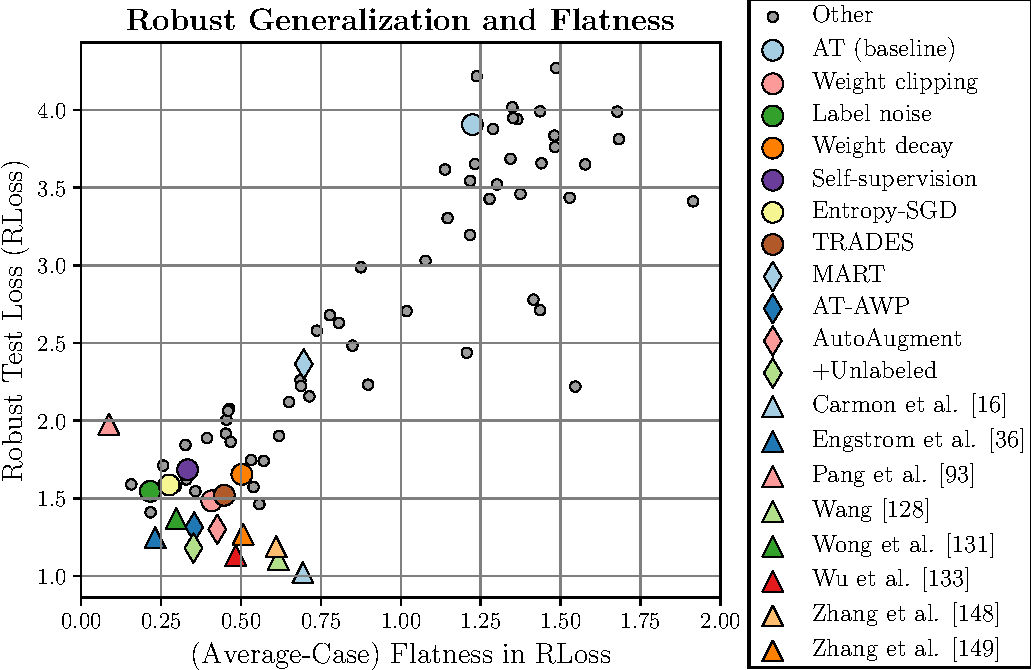
\includegraphics[width=0.5\textwidth]{plots_contributions_arxiv}
	\vspace*{-18px}
	\caption{\textbf{Robust Generalization and Flatness:} Robust loss (\RCE, lower is more robust, y-axis), \ie, cross-entropy loss on PGD adversarial examples \cite{MadryICLR2018}, against our \emph{average-case flatness} measure of \RCE in weight space (lower is ``flatter'', x-axis).
	Popular AT variants improving adversarial robustness on \CifarT, \eg, TRADES \cite{ZhangICML2019}, AT-AWP \cite{WuNIPS2020}, MART \cite{WangICLR2020} or AT with self-supervision \cite{HendrycksNIPS2019}/unlabeled examples \cite{CarmonNIPS2019}, also correspond to flatter minima. Vice-versa, regularization explicitly improving flatness, \eg, Entropy-SGD \cite{ChaudhariICLR2017}, weight decay or weight clipping \cite{StutzMLSYS2021}, also improve robustness.
	Across all models, there is a \textbf{clear relationship between good robust generalization and flatness in \RCE.}
	{\LARGE$\bullet$},\raisebox{0.5mm}{$\mathbin{\blacklozenge}$} Our models, \underline{w/o} early stopping.
	{\large$\blacktriangle$} RobustBench \cite{CroceARXIV2020b} models \emph{w/} early stopping.}
	\label{fig:introduction}
	\vspace*{-6px} 
\end{figure}

In order to obtain robustness against adversarial examples \cite{SzegedyICLR2014}, \emph{adversarial training (AT)} \cite{MadryICLR2018} augments training with adversarial examples that are generated on-the-fly. While many different variants have been proposed, AT is known to require more training data \cite{KhouryARXIV2018,SchmidtNIPS2018}, generally leading to generalization problems \cite{FarniaICLR2019}. In fact, \emph{robust overfitting} \cite{RiceICML2020} has been identified as the main problem in AT:  adversarial robustness on test examples eventually starts to decrease, while robustness on training examples continues to increase (\cf \figref{fig:main-overfitting}). This is typically observed as increasing \emph{robust loss (\RCE)} or \emph{robust test error (\RTE)}, \ie, (cross-entropy) loss and test error on adversarial examples. As a result, the \emph{robust generalization gap}, \ie, the difference between test and training robustness, tends to be very large. In \cite{RiceICML2020}, early stopping is used as a simple and effective strategy to avoid robust overfitting. However, despite recent work tackling robust overfitting \cite{SinglaARXIV2021,WuNIPS2020,HwangARXIV2020}, it remains an open and poorly understood problem.

In \emph{``clean''} generalization (\ie, on natural examples), overfitting is well-studied and commonly tied to flatness of the loss landscape in weight space, both visually \cite{LiNIPS2018} and empirically \cite{NeyshaburNIPS2017,KeskarICLR2017,JiangICLR2020}.
In general, the optimal weights on test examples do not coincide with the minimum found on training examples. Flatness ensures that the loss does \emph{not} increase significantly in a neighborhood around the found minimum. Therefore, flatness leads to good generalization because the loss on test examples does not increase significantly (\ie, small generalization gap, \cf \figref{fig:main-illustration}, right).
\cite{LiNIPS2018} showed that \emph{visually} flatter minima correspond to better generalization. \cite{NeyshaburNIPS2017} and \cite{KeskarICLR2017} formalize this idea by measuring the change in loss within a local neighborhood around the minimum considering random \cite{NeyshaburNIPS2017} or ``adversarial'' weight perturbations \cite{KeskarICLR2017}.
These measures are shown to be effective in predicting generalization in a recent large-scale empirical study \cite{JiangICLR2020} and explicitly encouraging flatness during training has been shown to be successful in practice \cite{ZhengARXIV2020c,CicekICCVWOR2019,TinICLR2020,ChaudhariICLR2017,IzmailovUAI2018}.

Recently, \cite{WuNIPS2020} applied the idea of flat minima to AT: through \emph{adversarial weight perturbations}, AT is regularized to find flatter minima of the \emph{robust} loss landscape. This reduces the impact of robust overfitting and improves robust generalization, but does not \emph{avoid} robust overfitting. As result, early stopping is still necessary. Furthermore, flatness is only assessed \emph{visually} and it remains unclear whether flatness does actually improve in these adversarial weight directions.
Similarly, \cite{GowalARXIV2020} shows that weight averaging \cite{IzmailovUAI2018} can improve robust generalization, indicating that flatness might be beneficial in general. This raises the question whether other ``tricks'' \cite{PangARXIV2020b,GowalARXIV2020}, \eg, different activation functions \cite{SinglaARXIV2021} or label smoothing \cite{SzegedyCVPR2016}, or approaches such as AT with self-supervision \cite{HendrycksNIPS2019}/unlabeled examples \cite{CarmonNIPS2019} are successful \emph{because of} finding flatter minima.

\begin{figure}[t]
	\centering
	\vspace*{-0.2cm}
	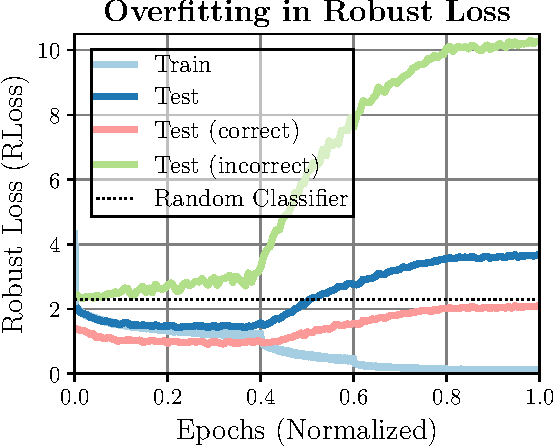
\includegraphics[width=0.225\textwidth]{plots_short_introduction_overfitting1}
	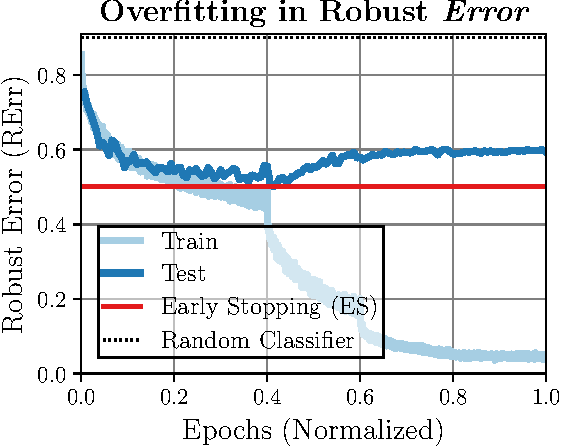
\includegraphics[width=0.225\textwidth]{plots_short_introduction_overfitting2}
	\vspace*{-8px}
	\caption{\textbf{Robust Overfitting:} Robust (cross-entropy) loss (\RCE) and robust error (\RTE) over epochs (normalized by $150$ epochs) for AT, \red{using a ResNet-18 on \CifarT (\cf \secref{sec:experiments})}, to illustrate \emph{robust} overfitting. \textbf{Left:} Training \RCE ({\color{plot0}light blue}) reduces continuously throughout training, while test \RCE ({\color{plot1}dark blue}) eventually increases again.
	We also highlight that robust overfitting is \emph{not} limited to incorrectly classified examples ({\color{plot4}green}), but also affects correctly classified ones ({\color{plot2}rose}). \textbf{Right:} Similar behavior, but less pronounced, can be observed considering \RTE. We also show \RTE obtained through early stopping ({\color{plot5}red}).}
	\label{fig:main-overfitting}
	\vspace*{-6px}
\end{figure}

\textbf{Contributions:} In this paper, we study \textbf{whether flatness of the robust loss (\RCE) in weight space improves robust generalization}. To this end,
we propose both average- and worst-case flatness measures for the \emph{robust} case, \red{thereby addressing challenges such as scale-invariance \cite{DinhICML2017}, estimation of \RCE on top or jointly with weight perturbations, and the discrepancy between \RCE and \RTE}. We show that \textbf{robust generalization generally improves alongside flatness} and vice-versa: \figref{fig:introduction} plots \RCE (lower is more robust, y-axis) against our average-case flatness in \RCE (lower is flatter, x-axis), showing a clear relationship. 
\red{In contrast to \cite{WuNIPS2020}, not providing empirical flatness measures, our results show that this relationship is stronger for average-case flatness.}
This trend covers a wide range of AT variants on \CifarT, \eg,  AT-AWP \cite{WuNIPS2020}, TRADES \cite{ZhangICML2019}, MART \cite{WangICLR2020}, AT with self-supervision \cite{HendrycksNIPS2019} or additional unlabeled examples \cite{CarmonNIPS2019,UesatoNIPS2019}, as well as various regularization schemes, including AutoAugment \cite{CubukARXIV2018}, label smoothing \cite{SzegedyCVPR2016} and noise or weight clipping \cite{StutzMLSYS2021}. Furthermore, we consider hyper-parameters, \eg, learning rate schedule, weight decay, batch size, or different activation functions \cite{ElfwingNN2018,MisraBMVC2020,HendrycksARXIV2016}, and methods explicitly improving flatness, \eg, Entropy-SGD \cite{ChaudhariICLR2017} or weight averaging \cite{IzmailovUAI2018}.